\documentclass[10pt,conference]{IEEEtran}
\usepackage{cite}
\usepackage{amsmath,amssymb}
\usepackage[hidelinks]{hyperref}
\usepackage{booktabs}
\usepackage{array}
\usepackage{graphicx}
\usepackage{algorithmic}
\usepackage{tikz}
\usetikzlibrary{arrows.meta,positioning,shapes.geometric}
\input{claim_macros}

\newtheorem{definition}{Definition}
\newtheorem{lemma}{Lemma}
\newtheorem{theorem}{Theorem}
\newcommand{\Allow}{\mathsf{ALLOW}}
\newcommand{\Deny}{\mathsf{DENY}}
\newcommand{\Err}{\mathsf{ERR}}
\newcommand{\Eval}{\mathcal{E}}
\newcommand{\Pol}{\mathcal{P}}
\newcommand{\Req}{\mathcal{Q}}
\newcommand{\Rel}{\mathcal{R}}
\newcommand{\Obl}{\mathcal{O}}
\newcommand{\Pass}{\mathsf{pass}}
\newcommand{\Reject}{\mathsf{reject}}
\newcommand{\Unsup}{\mathsf{unsupported}}
\newcommand{\Core}{\mathsf{Core}}

\title{LatticeGuard: Law-Guided Regression Oracles for Access-Control Evaluators}
\author{Anonymous Author(s)}

\begin{document}
\maketitle

\begin{abstract}
Access-control policy evaluators regress when authorization engines add features, optimize semantics, or refactor policy support, yet developers rarely have complete decision tables for every principal, action, and resource.  They usually know laws--deny dominance, default deny, hierarchy preservation, off-slice renaming--but not a hand-written oracle for every transformed request.  LatticeGuard converts these laws into executable metamorphic obligations and attaches an applicability predicate to each obligation, so a candidate is counted only when the concrete before/after pair is comparable, valid, and inside declared language support.  Sensitivity is exercised first: \LGSeededRows{} seeded semantic-drift controls produce a \LGSeededKillRate{}\% positive-control kill rate and \LGCounterexamples{} minimized replayable counterexamples.  The release-gating run then evaluates \LGPrimaryObligations{} applicable obligations over Casbin and Cedar native fragments plus an OPA/Rego normalized-decision fragment, with \LGPrimaryFailures{} primary backend failures, \LGRejected{} rejected invalid transformations, and \LGUnsupported{} unsupported fragments kept outside the denominator.  The contribution is not a bug claim or a pooled success rate; it is an evidence boundary that makes a clean evaluator run reviewable through applicability, rejection, theory replay, minimization, deployed-test comparison, and conservative denominator accounting.
\end{abstract}

\begin{IEEEkeywords}
access control, policy evaluation, metamorphic testing, regression oracle, authorization, reproducibility
\end{IEEEkeywords}

\section{Introduction}
Access-control policies evolve continuously: teams add denies, restructure role hierarchies, split resource scopes, rename policy atoms, or upgrade an evaluator.  Each edit can preserve, reduce, or intentionally change an authorization decision.  Yet developers seldom possess a complete oracle for every principal/action/resource request after every edit.  They instead reason with laws: default deny should remain deny when no matching rule becomes reachable; a matching forbid should dominate a matching permit; adding an already implied hierarchy edge should not change a decision; and an off-slice alpha-renaming should be observationally irrelevant.

The problem is not simply missing tests.  It is an oracle problem in a semantic domain where invalid transformations are easy to generate.  Metamorphic testing was designed for settings in which individual expected outputs are unavailable \cite{segura2016survey}; cybersecurity and logic-engine studies show why that idea is attractive beyond numerical programs \cite{chen2016mtcybersecurity} \cite{mansur2023datalog}.  Differential testing offers a parallel lesson: McKeeman's compiler formulation \cite{mckeeman1998differential}, Csmith \cite{yang2011csmith}, equivalence-modulo-input validation \cite{le2014emi}, and Nezha \cite{petsios2017nezha} all make disagreement useful only when the generated cases are meaningful.  Access-control policies make that last condition fragile.  A random extension can become reachable from the request principal; a renaming can touch the queried resource; a rule permutation can cross into a priority-sensitive fragment.  Counting such cases as passed metamorphic tests creates a convincing but false denominator.

LatticeGuard's thesis is that access-control laws should be compiled into obligations whose applicability can be checked.  Consider adding a deny rule for suspended users.  The law is not merely ``the edited policy should deny more requests.''  It applies only when the new deny is reachable for the same request slice and when no unrelated role or resource edit changes the comparison.  LatticeGuard records that side condition as part of the obligation.  A candidate contributes to the measured pass denominator only if its predicate establishes that the law applies to the concrete before/after pair.  Invalid candidates remain visible as rejected evidence; unsupported language fragments remain visible as unsupported evidence; neither can inflate results.

This design targets policy \emph{evaluators}, not policy authoring assistants.  The research object is the evaluator's treatment of deny/allow composition, request reachability, role/resource closure, shadowing, monotonicity, dominance, and refactoring-preserving transformations.  Casbin contributes a model/effect structure and native role matcher language \cite{casbin_model_docs} \cite{casbin_effect_docs}; Cedar contributes a PARC request model with forbid-overrides-permit semantics \cite{cedar_authz_docs} \cite{cedar_request_docs}; OPA/Rego is used only as a normalized-decision fragment over a law object \cite{opa_language_docs} \cite{opa_cli_docs}.  The counted evidence is CPU-local, offline-replayable, and frozen before claim generation, so the paper's contribution is not a bug story in one engine but a reusable law-to-obligation method.

Together, these pieces make denominator admission the object of evaluation rather than a reporting detail.  The paper contributes:
\begin{itemize}
\item \textbf{Law-level obligation model.} We define a typed evidence object for access-control metamorphic testing with executable applicability, rejection, unsupported-fragment, invariant, and minimization components.
\item \textbf{Soundness discipline.} We identify deny-aware monotonicity as a necessary condition for principal-order obligations and certify \LGRelations{} relation theorems, 48 proof obligations, \LGModelCheckCases{} finite core law instantiations, and \LGMechanizedKernelCases{} independent law-kernel replay cases.
\item \textbf{Evidence-chain implementation.} We build a deterministic research system that connects public/native policy material, evaluator calls, reference semantics, bounded law certificates, semantic counterexample replay, deployed-tool crosswalks, baseline interpretation, claim traceability, dependency provenance, and reproducibility checks.
\item \textbf{Evaluation.} On \LGSources{} frozen sources, LatticeGuard evaluates \LGPrimaryObligations{} applicable obligations over Casbin/Cedar native fragments and an OPA/Rego normalized-decision fragment with \LGPrimaryFailures{} primary failures, rejects \LGRejected{} invalid transformations, records \LGUnsupported{} unsupported rows, and produces \LGCounterexamples{} minimized positive-control witnesses.
\end{itemize}

\section{Problem Setting and Scope}
\label{sec:problem}
A policy evaluator maps a policy $P$ and request $q=(p,a,r,c)$ to a decision.  Casbin separates request definition, policy definition, effect, and matcher clauses \cite{casbin_model_docs}; its RBAC and priority material make role closure and order-sensitive evaluation explicit \cite{casbin_rbac_docs} \cite{casbin_priority_docs}.  Cedar evaluates a principal/action/resource/context request against permit and forbid policies with forbid precedence and default deny \cite{cedar_authz_docs}; its entity and schema material define the graph and type boundaries that a regression oracle must respect \cite{cedar_entities_docs} \cite{cedar_schema_docs}.  These languages expose different syntax and feature sets, but many regression risks are law-shaped.

\subsection{Motivating task}
Suppose a maintainer adds an explicit deny for suspended users, refactors a viewer/editor/owner hierarchy, and then upgrades an evaluator.  A conventional unit test can check one request.  It cannot easily state that the refactoring preserves all request slices whose role closure is unchanged, or that a new deny should dominate an existing allow exactly when it matches the same slice.  A differential test can compare two evaluators, but it does not explain whether disagreement reflects a real semantic drift, unsupported language mismatch, or an invalid test transformation.  LatticeGuard therefore treats the developer task as follows: from a law $\ell$, a policy slice $s$, and an adapter $A$, generate an obligation $o$ whose applicability can be independently recomputed.

\begin{definition}[Policy-slice obligation]
An obligation is a tuple
$\langle \ell,P,q,P',q',\pi_\ell,\rho_\ell,u_\ell,I_\ell,m_\ell\rangle$ where $\pi_\ell$ is the applicability predicate, $\rho_\ell$ rejects invalid transformations, $u_\ell$ marks unsupported fragments, $I_\ell$ is the expected decision invariant, and $m_\ell$ is the minimization recipe for failures.
\end{definition}

This definition is intentionally stricter than ordinary mutation testing.  A candidate that violates $\pi_\ell$ is not a failed obligation; it is a rejected oracle candidate.  That distinction is the difference between a trustworthy regression oracle and a mutation generator that tests its own accidental edits.

\subsection{Validity risks}
The validity risks are concrete: the law may be unsound, the predicate may be label-driven rather than recomputed, the corpus may be synthetic, the adapter boundary may be too broad, the denominator may hide rejections, the counterexample path may be unexercised, or the paper may overstate a zero-failure result.  LatticeGuard responds with evidence rather than reassurance.  Predicates are recomputed from policy/request material; native policy material is checked before normalization; primary, rejected, unsupported, seeded, and proof-obligation rows are kept as disjoint evidence classes.

\section{Law-Level Obligation Model}
\label{sec:model}
The core semantics abstracts an evaluator into a decision function $\Eval_A(P,q)\in\{\Allow,\Deny,\Err\}$.  The supported core contains principals, roles, resources, actions, role inheritance, allow rules, deny rules, and deny-overrides composition.  Let $\mathsf{cl}_P(p)$ denote the role closure reachable from principal $p$ in policy $P$, and let $\mathsf{match}_P(r,q)$ hold when rule $r$ is reachable from the principal and matches the action/resource slice.

\begin{definition}[Deny-overrides reference core]
The reference decision is $\Deny$ if any matching deny exists; otherwise $\Allow$ if any matching allow exists; otherwise $\Deny$.  A law predicate is sound for the core when every counted candidate satisfying the predicate also satisfies its invariant under this reference decision.
\end{definition}

The model is not a replacement for evaluator backends.  It is a guardrail for the oracle catalog.  Each law is first checked against the reference core, then exercised against declared backend fragments.  This two-level design prevents a relation from being admitted merely because a current implementation happens to agree with itself.

\begin{table*}[t]
\centering
\caption{Law catalog.  Each row is materialized as executable predicate, invariant, rejection rule, and minimization recipe.}
\label{tab:relations}
\begin{tabular}{p{0.05\linewidth}p{0.18\linewidth}p{0.31\linewidth}p{0.36\linewidth}}
\toprule
ID & Law family & Counted invariant & Predicate rejects when \\
\midrule
DD & Default deny & no reachable allow/deny remains deny & a new rule becomes reachable for the request \\
DO & Deny dominance & matching deny dominates matching allow & added deny does not match the same request slice \\
PA & Deny-aware principal monotonicity & allow preserved under role-closure superset and no new deny & closure is incomparable or a new deny interferes \\
DA & Deny antitonicity & reachable deny remains deny under substitution & deny witness is lost after substitution \\
IE & Irrelevant extension & unreachable extension preserves decision & extension touches principal/action/resource closure \\
ID & Idempotence & duplicate equivalent material preserves decision & duplicate is not semantically identical \\
HC & Hierarchy closure & implied edge preserves decision & inserted edge changes request-relevant closure \\
HR & Hierarchy refactoring & consistent child-role rewrite preserves decision & rewritten assignment does not preserve closure/decision \\
SR & Shadowed rule removal & removing dominated allow preserves deny & removed allow is not dominated by matching deny \\
RO & Rule-order invariance & unordered fragments preserve decision under permutation & priority or first/last-match semantics are present \\
AR & Alpha renaming & injective off-slice renaming preserves decision & renaming touches requested principal/resource/action \\
SM & Scope split/merge & equivalent scope partition preserves decision & matched resource/action set changes \\
\bottomrule
\end{tabular}
\end{table*}

\begin{lemma}[Denominator integrity]
A row contributes to the pass denominator iff its computed status is $\mathsf{APPLICABLE\_EVALUATED}$ and its before/after adapter decisions satisfy the declared invariant.  Rows with computed statuses $\mathsf{REJECTED\_NOT\_COUNTED}$, $\mathsf{UNSUPPORTED\_NOT\_COUNTED}$, $\mathsf{ERROR\_RECORDED}$, or $\mathsf{TIMEOUT\_RECORDED}$ cannot be counted as passes.
\end{lemma}

The admission rule is frozen before backend outcomes are interpreted.  Each relation contract names its predicate, invariant, rejection rule, and minimizer; each candidate receives a predicate-input hash and witness hash before it can reach the counted stream.  The predicate is allowed to consult the reference core to decide law side conditions, but it does not read adapter outcomes or generated result ledgers.  Candidates rejected by the predicate or support boundary retain rejection/support evidence but no before/after adapter outcome, so they cannot be promoted or demoted after a backend result is observed.

\begin{lemma}[Deny-aware principal monotonicity]
Under deny-overrides semantics, an allow decision is preserved by substituting a principal with a role-closure superset only if the follow-up slice has no newly matching deny.  Without the no-new-deny side condition, the law is unsound.
\end{lemma}

\noindent The second lemma is not cosmetic.  Negative PA witnesses show that a closure-superset predicate alone is insufficient: a larger closure can introduce a matching deny.  The frozen PA predicate therefore requires both a closure superset and absence of follow-up deny interference.

\begin{theorem}[Bounded core law certificate]
For the finite core bound used in the study--three roles, two users, one action, one resource, acyclic role inheritance, representative role assignments, and rules up to the frozen bound--all \LGRelations{} relation families have theorem rows whose side conditions discharge 48 executable proof obligations and satisfy their declared invariants for every counted candidate generated by their predicates.
\end{theorem}

\noindent The theorem is reported as an executable certificate rather than as an informal proof sketch only.  The checker enumerates finite policies and requests, applies each relation generator and predicate, checks the invariant against the reference core, and emits a digest over relation contracts, soundness rows, theorem rows, proof-obligation rows, and the model summary.  The current run checks \LGModelCheckCases{} cases with \LGModelCheckFailures{} failures and 48 discharged proof obligations.  The bound is finite, but the workflow matters: any future relation change must pass the same certificate before it can enter the primary denominator.


\subsection{Proof obligations behind the laws}
A relation family is admitted only after four obligations are discharged.  First, the generator must expose the syntactic edit it made, such as adding a deny, splitting a scope, or replacing a role assignment.  Second, the predicate must recompute semantic reachability from the concrete before/after policies; it cannot rely on a label supplied by the generator.  Third, the invariant must be checked against both the reference core and the backend decision pair.  Fourth, the minimizer must preserve the same predicate witness while deleting irrelevant policy material.  These obligations are intentionally redundant.  If a generator bug produces an invalid follow-up policy, the predicate rejects it.  If a predicate is too weak, the reference checker can expose a counterexample.  If a backend disagrees, the minimizer produces the smallest replayable slice that still satisfies the predicate.

\begin{table}[t]
\centering
\caption{Proof-certificate components.}
\label{tab:proofcert}
\begin{tabular}{p{0.30\linewidth}p{0.54\linewidth}}
\toprule
Component & Evidence check \\
\midrule
Predicate witness & why the law applies to this before/after pair \\
Theorem ledger & 12 relation theorem rows and 48 proof obligations \\
Reference replay & whether the law is sound in the bounded core \\
Backend replay & whether each declared backend fragment satisfies the invariant \\
Minimized witness & whether irrelevant policy material was removed without changing the failing law slice \\
\bottomrule
\end{tabular}
\end{table}

This structure is why LatticeGuard treats theory and execution as one argument.  The formal model rules out invalid law definitions; the adapter layer rules out vacuous formalism; the source provenance rules out hidden benchmark construction; and the claim checks rule out paper-only arithmetic.  A reader can question any edge in the chain and find a corresponding evidence class rather than a prose assurance.

\subsection{Obligation generation and minimization}
\label{sec:algorithm}
LatticeGuard follows a generate--filter--evaluate--minimize pipeline.  The generator proposes candidates from frozen subjects.  The predicate engine recomputes applicability from the before/after policies and requests.  Adapter execution happens only after applicability and unsupported-fragment checks.  Failures are minimized with relation-specific reducers.

\begin{figure}[t]
\centering
\begin{algorithmic}[1]
\REQUIRE subjects $S$, adapters $A$, relation contracts $L$
\FORALL{$s\in S$, $\ell\in L$}
  \STATE propose candidate $(P,q,P',q')$ for relation $\ell$
  \STATE compute $\rho_\ell$, $u_\ell$, and $\pi_\ell$ from policy/request material
  \IF{$\rho_\ell$ holds} \STATE record rejected, not counted; \textbf{continue} \ENDIF
  \IF{$u_\ell$ holds} \STATE record unsupported, not counted; \textbf{continue} \ENDIF
  \IF{not $\pi_\ell$} \STATE record rejected, not counted; \textbf{continue} \ENDIF
  \FORALL{$A_i\in A$}
    \STATE evaluate $d=\Eval_{A_i}(P,q)$ and $d'=\Eval_{A_i}(P',q')$
    \IF{$I_\ell(d,d')$} \STATE record pass with fixture hashes
    \ELSE \STATE minimize and write replay witness
    \ENDIF
  \ENDFOR
\ENDFOR
\end{algorithmic}
\caption{Obligation generation.  Predicate computation precedes adapter decisions and denominator accounting.}
\label{fig:algorithm}
\end{figure}

\begin{figure*}[t]
\centering
\begin{tikzpicture}[x=1cm,y=1cm,
  lgbox/.style={rectangle, draw=black!68, rounded corners=2pt, align=center,
    minimum height=0.82cm, text width=2.35cm, inner xsep=3pt, inner ysep=2.1pt,
    fill=black!3,
    text height=1.45ex, text depth=.34ex,
    font=\rmfamily\fontsize{7.0}{7.8}\selectfont},
  lggate/.style={diamond, aspect=2.1, draw=black!72, align=center,
    minimum height=0.88cm, text width=1.95cm, inner sep=1.5pt,
    fill=black!8, text height=1.45ex, text depth=.34ex,
    font=\rmfamily\fontsize{6.8}{7.5}\selectfont},
  lgnote/.style={rectangle, draw=black!35, rounded corners=1.5pt, align=center,
    minimum height=0.54cm, text width=2.2cm, inner xsep=2pt, inner ysep=1.8pt,
    fill=black!1, text height=1.25ex, text depth=.28ex,
    font=\rmfamily\fontsize{6.5}{7.1}\selectfont},
  lgarrow/.style={-Latex, line width=0.62pt, draw=black!68, line cap=round, line join=round},
  lgsoft/.style={-Latex, line width=0.48pt, draw=black!46, line cap=round, line join=round}]
\node[lgbox] (subjects) at (0,1.5) {\LGSources{} subjects\\official/native};
\node[lgbox] (contract) at (2.9,1.5) {law contract\\$\ell,\pi_\ell,\rho_\ell,u_\ell$};
\node[lggate] (gate) at (5.8,1.5) {admit?\\predicate};
\node[lgbox] (eval) at (8.7,1.5) {\LGPrimaryObligations{} applicable\\adapter replay};
\node[lgbox] (pass) at (11.6,1.5) {\LGPrimaryPasses{} passes\\\LGPrimaryFailures{} primary failures};
\node[lgbox] (claim) at (14.5,1.5) {bounded claim\\reviewable run};
\node[lgnote] (reject) at (4.45,0.10) {\LGRejected{} rejected\\invalid law edit};
\node[lgnote] (unsup) at (7.15,0.10) {\LGUnsupported{} unsupported\\outside fragment};
\node[lgnote] (seed) at (10.25,0.10) {\LGSeededRows{} seeded drifts\\\LGCounterexamples{} replays};
\node[lgnote] (audit) at (13.25,0.10) {denominator\\stays auditable};
\draw[lgarrow] (subjects) -- (contract);
\draw[lgarrow] (contract) -- (gate);
\draw[lgarrow] (gate) -- (eval);
\draw[lgarrow] (eval) -- (pass);
\draw[lgarrow] (pass) -- (claim);
\draw[lgsoft] (gate.south west) .. controls +(0,-0.65) and +(0,0.55) .. (reject.north);
\draw[lgsoft] (gate.south east) .. controls +(0,-0.65) and +(0,0.55) .. (unsup.north);
\draw[lgsoft] (eval.south) .. controls +(0,-0.65) and +(0,0.55) .. (seed.north);
\draw[lgsoft] (claim.south) .. controls +(0,-0.65) and +(0,0.55) .. (audit.north);
\end{tikzpicture}
\caption{Evidence flow.  A law contract becomes a counted regression row only after the predicate gate admits the before/after slice; rejected edits, unsupported fragments, and seeded controls remain visible but outside the primary pass denominator.}
\label{fig:flow}
\end{figure*}

The minimizer is law-aware.  A deny-dominance failure is reduced to the matching allow, matching deny, and request.  A hierarchy failure keeps the edge witness and closure-relevant request.  A scope split/merge failure keeps the partition and matched action/resource set.  This design yields small counterexamples with semantics attached, not opaque failures.  It also lets a maintainer replay one failure family without rerunning the full experiment.

\section{Evidence Construction}
\label{sec:evidence}
LatticeGuard is implemented as an end-to-end research system rather than as a monolithic test generator.  Its components connect law algebra, evaluator adapters, benchmark import, source linkage, proof certificates, counterexample replay, and claim checking.  The implementation checks not only reported counts but also schema contracts, native fixture self-tests, predicate witnesses, counterexample families, result invariants, dependency provenance, import closure, and anonymization.


\begin{table}[t]
\centering
\caption{Evidence-chain hardening.}
\label{tab:repo}
\begin{tabular}{p{0.39\linewidth}p{0.46\linewidth}}
\toprule
Dimension & Verifier-visible evidence \\
\midrule
Evaluator execution & \LGNativeAdapters{} native adapters plus \LGDecisionHarnesses{} normalized decision harness with \LGPrimaryObligations{} applicable obligations \\
Invalid-oracle discipline & \LGRejected{} rejected candidates and \LGUnsupported{} unsupported rows outside the pass denominator \\
Positive-control replay & \LGSeededRows{} seeded rows, \LGSeededKilled{} killed, and \LGCounterexamples{} minimized counterexamples \\
Native fixture evidence & \LGNativeSelftests{} raw native self-tests with \LGNativeFailures{} failures \\
Bounded law certificate & \LGModelCheckCases{} checked cases, 12 theorem rows, and 48 proof obligations \\
Claim binding & \LGAggregateChecks{} consistency checks over frozen evidence, claims, and replay traces \\
\bottomrule
\end{tabular}
\end{table}

\subsection{Adapters}
The counted evidence uses unequal fragment roles.  Casbin and Cedar are exercised through native evaluator semantics for the admitted slice; OPA/Rego is exercised only as a normalized-decision harness over a law object whose hierarchy closure is supplied by the reference core.  The evaluated packet therefore contains \LGNativeAdapters{} native adapters and \LGDecisionHarnesses{} supplied-closure decision harness, not three interchangeable native backends.

\emph{Adapter boundary.}  For hierarchy stress cases, OPA/Rego receives precomputed reachable roles from LatticeGuard's trusted semantic core; Rego then executes the normalized allow/deny decision over that closure.  We count OPA as a decision harness for the normalized fragment, not as evidence that recursive hierarchy closure is implemented natively in Rego.  Thus hierarchy-sensitive OPA rows are normalized-fragment evidence, while Casbin and Cedar rows also exercise native hierarchy machinery in the admitted slice.  Each role declares its supported fragment, decision normalization, hierarchy mapping, and material digests before entering denominators.

\subsection{Benchmark funnel}
The benchmark funnel has five explicitly separated strata.  First, \LGOfficialDocSources{} documentation-derived slices are transcribed from official Casbin/Cedar semantics and OPA/Rego normalized-fragment semantics.  Second, \LGUpstreamExampleSources{} upstream example slices are canonicalized from public project material.  Third, \LGNativeCanonicalSources{} native canonical slices are imported only after raw native self-tests.  Fourth, \LGStressWitnessSources{} semantic stress witnesses exercise relation combinations derived from the frozen law catalog and are internal hypothesis tests, not independent upstream benchmarks.  Fifth, \LGGeneratedSources{} generated canonical law probe remains explicitly labeled as generated.  The native layer executes \LGNativeSelftests{} raw self-tests with \LGNativeSelftestPasses{} passes before normalized law objects are evaluated.  External-validity claims are therefore attached to the public/native strata and self-tests, while stress witnesses test law-composition coverage.


\subsection{Native-to-canonical translation contract}
Native material creates a methodological risk: a translation can accidentally simplify the policy until the benchmark becomes a generated example again.  LatticeGuard therefore records three objects for every native bundle.  The raw object is the original model/policy/entity material.  The native self-test object is the decision table executed before normalization.  The canonical object is the translated policy slice used by relation generators.  The linkage check requires each canonical subject to point back to raw digests and each raw bundle to have at least one native self-test row.  This design makes the benchmark funnel inspectable without requiring readers to learn every adapter's syntax before understanding the experiment.

\begin{table}[t]
\centering
\caption{Benchmark funnel invariants.}
\label{tab:funnel}
\begin{tabular}{p{0.34\linewidth}p{0.50\linewidth}}
\toprule
Funnel stage & Required invariant \\
\midrule
Raw native material & source digest, declared source type, license, adapter family \\
Native self-test & raw decision executed before normalization \\
Canonical subject & link to raw bundle or explicit generated label \\
Relation candidate & source identifier preserved through predicate and adapter rows \\
Paper claim & numeric macro derived from checked result evidence, not manual count \\
\bottomrule
\end{tabular}
\end{table}

The resulting corpus is deliberately heterogeneous.  Some sources are official semantic slices, some are native fixture bundles, and one is a generated canonical law probe.  LatticeGuard keeps these strata separate because collapsing them would make the evidence look larger but less meaningful.  The claim we need for evaluator regression testing is not that every policy in the wild has been sampled; it is that law obligations can be generated, filtered, and replayed across public, native, and canonical material with the same denominator rules.

\begin{table}[t]
\centering
\caption{Current evidence summary.  Primary failures are release-gating failures; rejected and unsupported rows audit admission boundaries.}
\label{tab:results}
\begin{tabular}{lr}
\toprule
Metric & Value \\
\midrule
Native adapters plus decision harnesses & \LGNativeAdapters{}+\LGDecisionHarnesses{} \\
Subject sources & \LGSources{} \\
Documentation-derived slices & \LGOfficialDocSources{} \\
Upstream example slices & \LGUpstreamExampleSources{} \\
Native canonical slices & \LGNativeCanonicalSources{} \\
Semantic stress witnesses & \LGStressWitnessSources{} \\
Generated law probe & \LGGeneratedSources{} \\
Relation families & \LGRelations{} \\
Applicable primary obligations & \LGPrimaryObligations{} \\
Primary obligation passes & \LGPrimaryPasses{} \\
Primary backend failures & \LGPrimaryFailures{} \\
Rejected invalid transformations & \LGRejected{} \\
Unsupported fragments & \LGUnsupported{} \\
Seeded semantic-drift rows & \LGSeededRows{} \\
Killed seeded rows & \LGSeededKilled{} \\
Minimized counterexamples & \LGCounterexamples{} \\
Bounded model-check cases & \LGModelCheckCases{} \\
\bottomrule
\end{tabular}
\end{table}

\begin{figure}[t]
\centering
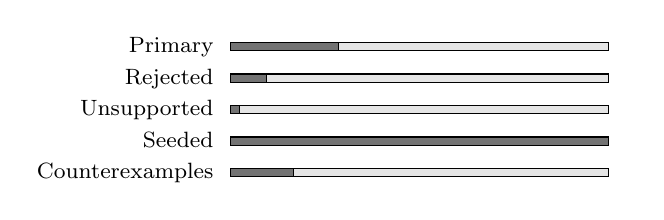
\begin{tikzpicture}[x=0.048cm,y=0.40cm]
\foreach \name/\w/\val/\y in {Primary/28.6/\LGPrimaryObligations/4,Rejected/9.5/\LGRejected/3,Unsupported/2.4/\LGUnsupported/2,Seeded/100/\LGSeededRows/1,Counterexamples/16.7/\LGCounterexamples/0}{
  \draw[fill=gray!20] (0,\y) rectangle (100,\y+0.26);
  \draw[fill=black!55] (0,\y) rectangle (\w,\y+0.26);
  \node[anchor=east,font=\footnotesize,text height=1.35ex,text depth=.28ex] at (-2,\y+0.13) {\name};
  \node[anchor=west,font=\footnotesize,text height=1.35ex,text depth=.28ex] at (102,\y+0.13) {\val};
}
\end{tikzpicture}
\caption{Claim-verified experimental scale.  Bar lengths are normalized to seeded control rows; labels show checked counts.}
\label{fig:evidencebars}
\end{figure}

\section{Results}
\label{sec:evaluation}
The evaluation asks five questions: RQ1, can executable predicates separate applicable obligations from invalid transformations? RQ2, do counted evaluator backends satisfy the law catalog over frozen subjects? RQ3, do seeded drifts exercise failure/minimization paths? RQ4, is the law catalog backed by executable theory rather than prose? RQ5, do deployed idioms and component ablations explain away the contribution?

The first reading of the evaluation is sensitivity, not a leaderboard score.  Seeded semantic drifts break deny precedence, hierarchy closure, forbid effects, permit stripping, and allow stripping so that the failure path must produce minimized witnesses.  The release-gating stream is interpreted under that positive-control evidence: if a backend honors the declared law over a supported fragment, the expected primary outcome is a pass; a failure would indicate semantic regression or wrapper/reference disagreement.  The primary result is \LGPrimaryPasses{}/\LGPrimaryObligations{} passes over pre-admitted obligations.  A denominator-pressure view pessimistically counts rejected and unsupported candidates against the run, yielding a \LGAllCandidatePassRate{}\% accounting view; it audits admission rather than replacing the primary rate.

\subsection{RQ1: applicability discipline}
The predicate engine computed \LGPredicateWitnesses{} candidate witnesses.  Of these, \LGPrimaryObligations{} adapter-level obligations entered the denominator; \LGRejected{} invalid transformations and \LGUnsupported{} unsupported fragments were separately reported.  The most important rejected families are default-deny candidates that add reachable allows, hierarchy transformations that reverse a parent relation, alpha-renamings that touch the requested principal, scope splits that drop the only matching permission, and rule-order tests in priority-sensitive fragments.  These are not failures of LatticeGuard; they are evidence that the oracle does not count unsound tests.

\subsection{RQ2: counted backend execution}
Table~\ref{tab:results} reports the primary execution.  Casbin and Cedar native fragments plus the OPA/Rego normalized-decision harness pass all \LGPrimaryObligations{} applicable obligations in the evaluated slice, with no primary errors or timeouts.  Cross-backend comparable rows have \LGCrossAdapterDiscrepancies{} discrepancies over \LGCrossAdapterComparable{} comparable decisions.  Zero discrepancies is expected on this normalized deny-overrides fragment because comparison is admitted only after support and validity filtering: \LGUnsupported{} unsupported rows and \LGRejected{} invalid transformations remain visible but do not enter the shared-fragment differential.  The result is a consistency check over the predeclared comparable subset, not evidence that the three roles have identical native semantics or complete language coverage.

\subsection{RQ3: seeded semantic drifts}
Because the current counted backends do not violate the evaluated obligations, the counterexample path is exercised with seeded semantic-drift evaluators.  The drift families cover precedence violations, hierarchy-closure loss, and accidental permission loss, which are the policy-regression patterns the law catalog is designed to isolate rather than a post hoc set of easy mutants.  LatticeGuard kills \LGSeededKilled{} of \LGSeededRows{} seeded rows and emits \LGCounterexamples{} minimized counterexamples.  The \LGSeededKillRate{}\% kill rate is intentionally lower than a program mutation score: same-stream point checks expose \LGSeededPointMismatches{} decision mismatches, but only \LGSeededHeadToHeadOverlap{} rows become law-level kills after the relation predicate admits them; the remaining point-only changes stay visible outside the law-failure claim.  A separate semantic replay re-evaluates every minimized witness from stored before/after request material and seeded-mutant semantics.

\subsection{RQ4: executable theory and coverage depth}
RQ4 has two parts: whether the laws have executable support and whether the subjects are nontrivial.  The theory side consists of 12 relation theorems, 48 proof obligations, \LGModelCheckCases{} bounded core cases, and \LGMechanizedKernelCases{} independent law-kernel replay cases over all 12 relation families.  The corpus side imports raw Casbin and Cedar material, checks native decisions, then normalizes the material into law-object subjects.  Coverage is measured across adapters, relation families, subject strata, and candidate statuses; every adapter/relation cell has applicable passes.

\begin{table}[t]
\centering
\caption{Quality challenges and evidence.  The responses are gate checks, not post hoc assurances.}
\label{tab:objections}
\begin{tabular}{p{0.32\linewidth}p{0.55\linewidth}}
\toprule
Objection & Response \\
\midrule
Predicates are labels & Predicate engine recomputes status and witness from policy/request material \\
Benchmark is shallow & \LGNativeSelftests{} raw native fixture self-tests plus \LGSources{} frozen sources \\
Denominator hides failures & Rejected/unsupported statuses are disjoint from pass denominator \\
Theory is informal & \LGModelCheckCases{} bounded cases, \LGMechanizedKernelCases{} kernel replays, and proof certificate \\
Counterexamples are not replayable & \LGCounterexamples{} minimized witnesses plus semantic replay evidence \\
Evidence is not independently checkable & Frozen theory, claim, source-linkage, hygiene, and replay ledgers agree \\
\bottomrule
\end{tabular}
\end{table}

\subsection{RQ5: baselines, replay, and claim verification}
RQ5 asks whether a simpler explanation suffices.  Policy test suites, request generators, differential checks, and mutation frameworks supply useful evidence, but they do not by themselves decide whether a transformation belongs in a law-level denominator.  We treat deployed-tool idioms as a nearest-neighbor comparison surface rather than as a single runnable substitute: native fixture tests, OPA-style policy-test decisions, XACML/RBAC request-generation idioms, cross-adapter differential checks, property-generation without rejection, release-pair prechecks, and the full law oracle are reported with their distinct admission rules.  We then use three baseline layers: a deployed-tool crosswalk over \LGDeployedCrosswalkRows{} idioms; a \LGDeployedHeadToHeadRows{}-row same-stream head-to-head over the same primary and seeded transformations as the law oracle; and component ablations that remove applicability, rejection, unsupported accounting, replay, native import, and bounded law certificates.  The frozen evidence spine ties those ledgers to protocol-freeze, claim-traceability, and integrity rows, and robustness replay reports zero mismatches.

The deployed comparison changes the interpretation of the zero-primary-failure result.  A clean run is not presented as superiority over deployed tests; those tests remain valuable at the decision level.  On the seeded stream, point tests can flag more raw decision mismatches than the law oracle admits, while every law-level seeded kill overlaps a same-stream point mismatch.  The claim is therefore not that point tests are useless, but that release-gating evidence needs an additional admission rule: before a decision comparison can become a regression-oracle row, the law predicate must establish that the follow-up policy should preserve or order the original decision, and any future violation must reduce to a replayable witness.


\subsection{Claim surface and failure policy}
The evaluation has a narrow but important failure policy.  A primary adapter failure is counted only when a row is applicable, supported, executable, and violates the declared invariant.  A rejected candidate is a success of the oracle filter, not a pass of the evaluator.  An unsupported candidate is evidence about adapter/language coverage, not evidence about correctness.  A timeout or adapter error is visible in the ledger and cannot be silently dropped.  These rules matter because a policy-testing paper can otherwise improve its headline number by deleting hard rows, moving invalid rows into passes, or changing the denominator after seeing results.

The reported numbers are intentionally few: applicable obligations, passes, rejections, unsupported rows, seeded rows, minimized counterexamples, native self-tests, bounded model cases, mechanized kernel cases, baseline families, and source counts.  All of them are generated from checked result evidence.  The supplementary material contains additional diagnostics, but the main paper avoids turning into a table dump.  This mirrors the intended developer workflow: the main result is the law-to-obligation mechanism; the detailed evidence remains the trace.

\subsection{End-to-end obligation traces}
The evaluation retains concrete traces for the obligations that matter most to maintainers: deny dominance, hierarchy refactoring, off-slice alpha renaming, and native-material import.  Each trace records the before/follow-up policy slice, request material, predicate witness, normalized adapter decisions, reference decisions, and any rejection reason.  Table~\ref{tab:rqmap} shows how these row-level traces answer the paper's research questions without forcing the main text to enumerate every trace.

\begin{table*}[t]
\centering
\caption{How each research question is answered by an executable evidence stream.}
\label{tab:rqmap}
\begin{tabular}{p{0.12\linewidth}p{0.26\linewidth}p{0.31\linewidth}p{0.21\linewidth}}
\toprule
RQ & Question & Evidence stream & Current outcome \\
\midrule
RQ1 & Are invalid transformations filtered before accounting? & predicate witnesses and rejection/unsupported evidence & \LGRejected{} rejected, \LGUnsupported{} unsupported \\
RQ2 & Do counted evaluator roles satisfy declared laws? & Casbin/Cedar native decisions plus OPA/Rego normalized-fragment decisions & \LGPrimaryPasses{}/\LGPrimaryObligations{} pass \\
RQ3 & Does the failure path work? & seeded semantic-drift evaluators and minimizers & \LGSeededKilled{} killed; \LGCounterexamples{} minimized \\
RQ4 & Is the law catalog more than prose? & theorems, proof obligations, bounded core, kernel replay & 12 theorem rows; 48 obligations; \LGMechanizedKernelCases{} kernel cases \\
RQ5 & Do simpler baselines explain the result? & \LGBaselineFamilies{} baseline families, \LGDeployedCrosswalkRows{} deployed idioms, \LGDeployedHeadToHeadRows{} same-stream comparisons, and claim binding & no simpler baseline supplies law admission, replay, and bounded support together \\
\bottomrule
\end{tabular}
\end{table*}

\subsection{Ablations and baselines}
\label{sec:baselines}
LatticeGuard is not positioned against a single end-to-end tool because the closest alternatives solve different oracle problems.  OPA and Cedar suites exercise expected decisions, XACML/RBAC generators build request sets, and mutation-testing systems mutate programs or tests; none decide whether an access-control transformation is applicable before it enters a regression-oracle denominator.  The deployed crosswalk records what these idioms contribute, while the same-stream head-to-head makes the comparison empirical at the decision-stream level: native and OPA-style point checks report zero failures on the clean primary stream, seeded point checks expose \LGSeededPointMismatches{} decision mismatches, and LatticeGuard admits \LGSeededHeadToHeadOverlap{} of those rows as law-level kills under the relation predicates.  We then compare against upstream-only, cross-adapter-only, random-without-rejection, single-relation, no-minimization, no-native-import, and no-bounded-certificate alternatives over the same frozen candidates.

The baselines show why the design is not reducible to more tests.  Point tests do not generate law obligations; cross-adapter disagreement is not an oracle without applicability; random mutation without rejection admits unsound rows; single-relation variants miss multi-causal drifts; removing native import weakens provenance; and removing the bounded checker reopens the PA monotonicity bug described in Section~\ref{sec:model}.


\subsection{Baseline design criteria}
The baselines were selected to be explanatory rather than ornamental.  A fair baseline must share the same subjects, adapters, and replay infrastructure; otherwise an improvement could come from easier inputs rather than a better oracle.  Each baseline removes one component from the evidence chain: predicate checks, rejection ledger, native material, minimization, or bounded law support.  The design follows oracle-problem evaluation practice from Barr et al. \cite{barr2015oracle} and Anand et al. \cite{anand2013orchestrated}.  It also borrows mutation-testing pressure from Ammann and Offutt's testing treatment \cite{ammann2016introduction}, Jia and Harman's survey \cite{jia2011mutation}, Papadakis et al.'s analysis \cite{papadakis2019mutation}, and Defects4J-style controlled bug evidence \cite{just2014mutants}.

The seeded semantic-drift family is the positive-control sensitivity test.  It does not pretend to be a discovered vulnerability.  Instead, it tests whether the method can produce a law-named, minimized counterexample when an evaluator violates deny dominance, hierarchy closure, forbid precedence, allow stripping, or permit stripping.  Without this control, a zero-failure primary run would leave the counterexample path untested.  With it, readers can inspect both the no-failure primary result and the live failure-reduction machinery.

\begin{table}[t]
\centering
\caption{Ablation logic over the seeded fault model.  Each ablation removes one admission or replay mechanism.}
\label{tab:ablations}
\begin{tabular}{p{0.35\linewidth}p{0.50\linewidth}}
\toprule
Ablation & Failure mode exposed \\
\midrule
No applicability predicate & invalid transformations enter denominator \\
No rejection evidence & denominator cannot be inspected \\
No unsupported accounting & skipped fragments masquerade as clean coverage \\
No replayable evidence & violations cannot be independently reconstructed \\
No native fixtures & public evidence becomes documentation-only \\
No bounded/kernel checker & unsound deny-oblivious PA law can be admitted \\
Single relation only & misses drift families outside that law \\
No minimization & failures are large and hard to replay \\
Cross-adapter only & disagreement lacks law-level explanation \\
\bottomrule
\end{tabular}
\end{table}

This baseline structure follows the evaluation logic of strong testing papers: the comparison isolates which mechanism accounts for the improvement, rather than merely reporting that a new tool found more examples.  It also clarifies the contribution boundary.  XACML request generation contributes systematic request construction \cite{bertolino2010systematic} and automated policy-test inputs \cite{bertolino2012xacmlrequests}.  Policy coverage metrics explain why request breadth matters \cite{martin2006coverage} and why quality cannot be reduced to syntax coverage \cite{martin2008quality}.  Multiple-implementation policy testing supplies a differential comparison surface \cite{li2008xacmlmultiple}; model-based policy tests add specification-driven test construction \cite{pretschner2008model}; verification and change-impact work explain why policy evolution needs semantic checks \cite{fisler2005verification} \cite{martin2007changeimpact}.

\subsection{Why these baselines are adversarial}
A weak evaluation would compare LatticeGuard only to no testing or to manually written examples.  We instead use baselines that try to explain away the contribution.  Upstream-only evidence asks whether public examples already expose seeded drifts; cross-adapter evidence asks whether disagreement alone is enough; random mutation asks whether any valid-looking edit can serve as a metamorphic oracle; and single-relation ablations ask whether one law family covers the drift space.  These alternatives fail for different reasons, which is the point: access-control evaluator regressions can occur in combination algorithms, role closure, shadowing, priority handling, or normalization.

\begin{table*}[t]
\centering
\caption{Baseline interpretation.  Rows compare simpler explanations over the same frozen evidence surface.}
\label{tab:baselineinterp}
\begin{tabular}{p{0.20\linewidth}p{0.32\linewidth}p{0.35\linewidth}}
\toprule
Baseline & Competing explanation & Why it is insufficient \\
\midrule
Native/OPA point tests & Deployed tests already cover the semantics & Same-stream point checks expose decision mismatches, but law predicates decide which rows become regression-oracle failures \\
Cross-adapter differential & Disagreement is enough as an oracle & Disagreement lacks applicability and invalid-transformation reasoning \\
Release-pair precheck & Version comparison is enough & A release pair becomes evidence only after the same applicability and replay gates admit it \\
Random valid mutation & More policy edits will find the same drifts & Valid-looking edits can change the request slice and poison the denominator \\
Single relation catalog & One strong relation family is enough & Drift families distribute across deny, hierarchy, shadow, order, and scope laws \\
No minimization & Failure detection is enough & Large failures are hard to replay and weakly explanatory \\
No bounded checker & Empirical rows establish law soundness & Empirical rows alone admitted the deny-oblivious PA predicate \\
\bottomrule
\end{tabular}
\end{table*}

\section{Discussion and Validity Boundaries}
\label{sec:implications}
The engineering shift is from point examples to regression obligations.  An example says whether one request is allowed or denied; a law obligation says which transformation should preserve or order a decision and why.  That distinction is what makes a regression row actionable: deny dominance, hierarchy closure, alpha-renaming, and scope split/merge each carry different side conditions and different counterexample explanations.  LatticeGuard therefore treats applicability predicates as the core software-engineering object, not as bookkeeping.  The denominator is decided by executable predicates, rejection rules, unsupported-fragment policy, reference agreement, and bounded semantic checks rather than by an after-the-fact spreadsheet.

The same structure makes failures interpretable without overclaiming.  A primary failure requires an applicable, supported, executable row whose invariant is violated; rejected candidates and unsupported fragments remain visible but do not become passes; seeded semantic drifts are positive controls rather than discovered vulnerabilities.  A maintainer can reuse the same object in release checking, policy refactoring, or language porting: freeze subjects, run the relevant law families, inspect only rows whose predicates and feature support make them comparable, and minimize any violation into replay material.

\subsection{Outcome semantics}
The outcome taxonomy is part of the method because access-control testing papers are easy to overstate.  If a tool reports only passes and failures, a reader cannot tell whether a transformation was valid, whether the adapter supported the fragment, whether a failure came from a real evaluator, or whether a seeded drift was being used as a positive control.  LatticeGuard therefore assigns every candidate to a mutually exclusive class before aggregation.  Counted rows require a predicate witness and adapter execution; excluded rows must carry a rejection or support reason; seeded rows remain separated from primary evidence.  This prevents three common mistakes: inflating the denominator with invalid edits, treating unsupported language fragments as successes, and presenting synthetic faults as discovered bugs.

\begin{table*}[t]
\centering
\caption{Outcome semantics used by the regression-oracle evidence chain.}
\label{tab:triage}
\begin{tabular}{p{0.18\linewidth}p{0.30\linewidth}p{0.39\linewidth}}
\toprule
Outcome class & Meaning & Evidence retained for inspection \\
\midrule
Applicable pass & Law predicate holds and invariant holds & before/after adapter decisions, predicate witness, fixture hashes \\
Primary failure & Law predicate holds and invariant fails & violated invariant, minimized counterexample, replay request \\
Rejected candidate & Candidate transformation is invalid for the law & rejection reason and witness; excluded from denominator \\
Unsupported fragment & Adapter or language fragment lies outside declared support & unsupported reason; excluded from denominator \\
Seeded drift kill & Known semantic drift violates a counted law & positive-control family and minimized replay material \\
Adapter exclusion & Evaluator path is not safely pinned before results & pre-result exclusion reason and pinning contract \\
\bottomrule
\end{tabular}
\end{table*}

This taxonomy also makes extension safer.  Adding an adapter is not merely adding another executable; it must declare fragment support, decision normalization, hierarchy handling, and provenance pins before it contributes to denominators.  Adding a law is not merely adding a transformation; it must define the predicate, invariant, rejection condition, unsupported-fragment behavior, and minimizer.  Adding sources is not merely increasing scale; each source must retain its stratum and raw linkage.  These requirements are deliberately strict because the paper's central claim is about trustworthy regression oracles, not about maximizing row counts.

\subsection{Maintainer workflow}
A maintainer uses LatticeGuard by selecting the law families relevant to an evaluator release or policy refactoring, freezing the subject corpus, and rerunning the corresponding obligations.  The output is not a raw disagreement list: each counted row has a law name, predicate witness, adapter decision pair, and minimization path.  This lets a team start with deny dominance, default deny, and irrelevant extension, then add hierarchy, shadowing, alpha-renaming, and scope laws as language support matures.

\subsection{Evidence chain as method}
For a regression-oracle paper, replayable evidence is not an appendix; it is part of the method.  The scientific object is a counted obligation, and that object only exists after several steps agree: a source slice is imported, raw native material is self-tested when available, a canonical subject is linked to its source, a law predicate admits a candidate, adapter executions produce normalized before/after decisions, the reference semantics agrees with the adapter decisions, and any violation can be minimized into replay material.  If one step is informal, the result becomes a tool report rather than an oracle discipline.

This design deliberately separates two notions that are often conflated.  Verification checks whether a reported claim follows from the released evidence.  Validation asks whether the claim is meaningful for evaluator maintenance.  LatticeGuard needs both.  Claim verification prevents stale counts and missing replay inputs from entering the release evidence.  Validation comes from the law catalog, native-material linkage, alternative baselines, seeded drifts, and bounded theory support.  Evidence can be reproducible but scientifically weak, or scientifically plausible but hard to reproduce; the contribution is stronger only when these dimensions are tied together.

\begin{table}[t]
\centering
\caption{Evidence-chain checks that support the main claims.}
\label{tab:evidencechain}
\begin{tabular}{p{0.36\linewidth}p{0.52\linewidth}}
\toprule
Evidence lens & Property checked before a claim is reported \\
\midrule
Claim traceability & visible counts match generated macros and claim rows \\
Predicate replay & computed status and witnesses are reproducible \\
Source linkage & raw, native, canonical, stress, and generated strata remain distinct \\
Proof support & relation laws have theorem rows, bounded cases, and kernel replay \\
Adapter agreement & counted decisions match executable reference semantics \\
Counterexample replay & minimized witnesses retain decision material \\
Dependency closure & imports resolve from declared pinned material \\
Hygiene and anonymity & transient, process, and identity residue are absent \\
\bottomrule
\end{tabular}
\end{table}

\subsection{Evidence-overfitting controls}
A common validity risk is to grow the dataset while leaving the oracle weak.  LatticeGuard uses four controls.  First, each relation must provide a predicate, invariant, rejection rule, unsupported-fragment rule, and minimizer before it can add counted rows.  Second, the benchmark funnel keeps documentation-derived slices, upstream examples, native imports, semantic stress witnesses, and generated probes as distinct strata.  Third, seeded drifts are generated independently of the primary adapter result; they can exercise the counterexample path but cannot turn a primary failure into a pass.  Fourth, the replay reports a hash-based source holdout, denominator-pressure accounting, and excluded-row checks showing rejected or unsupported rows retain no adapter outcomes.

\begin{table}[t]
\centering
\caption{Controls against common validity attacks.}
\label{tab:overfit}
\begin{tabular}{p{0.38\linewidth}p{0.48\linewidth}}
\toprule
Attack & Guardrail \\
\midrule
Grow easy rows after seeing results & frozen relation contracts and protocol amendment log \\
Move invalid rows into passes & executable predicate and denominator check \\
Hide unsupported language features & unsupported evidence with adapter support matrix \\
Overstate public benchmark depth & separated source strata and raw-hash linkage \\
Claim failure sensitivity without failures & seeded drift rows and minimization replay \\
Claim theory from examples & bounded core model checker, kernel replay, and proof certificate \\
Trust wrapper translation implicitly & adapter/reference agreement over every counted decision \\
Risk reference-integrity failure & citation and metadata consistency check \\
Perfect pass rate is overfit & outcome-independent holdout and denominator-pressure summaries \\
\bottomrule
\end{tabular}
\end{table}

\subsection{Reading a zero-primary-failure run}
A zero-primary-failure run is useful only if the denominator is inspectable.  It could mean the evaluated fragments satisfy the declared laws, or it could reflect weak laws, filtered unsupported cases, a tuned corpus, or a dead failure path.  LatticeGuard separates these readings by reporting applicable passes, rejections, unsupported fragments, seeded drifts, minimized counterexamples, model-check cases, baseline families, holdout coverage, and denominator-pressure summaries alongside the primary count.  The result should therefore be read as regression assurance over declared fragments, not as ``no access-control bugs exist'' or ``the engines are equivalent.''

\begin{table}[t]
\centering
\caption{Why a zero-primary-failure run is still reviewable.}
\label{tab:zerofailure}
\begin{tabular}{p{0.33\linewidth}p{0.53\linewidth}}
\toprule
Validity pressure & Evidence retained in the package \\
\midrule
Laws are vacuous & applicable, rejected, and unsupported rows remain separate \\
Adapters are wrappers & counted decisions are checked against reference semantics \\
Invalid edits were hidden & rejection witnesses stay in the released evidence \\
Unsupported features became passes & unsupported rows are reported outside denominators \\
Failure path was inert & seeded drifts produce minimized replay witnesses \\
Denominator was tuned & hash-based source split and source strata are fixed before aggregation \\
\bottomrule
\end{tabular}
\end{table}

The current run increases evidence depth without treating scale as evidence by itself: \LGPrimaryObligations{} applicable obligations, \LGRejected{} rejected transformations, \LGUnsupported{} unsupported fragments, \LGSeededRows{} seeded drift rows, \LGCounterexamples{} minimized counterexamples, \LGMechanizedKernelCases{} law-kernel replay cases, and \LGBaselineFamilies{} baseline families retain separate accounting roles.  Seeded semantic drifts show that broken law families produce minimized witnesses, while future release-pair or backend claims must enter through the same relation and adapter contracts.

This accounting also blocks two common overfitting readings.  First, a large clean denominator is not treated as evidence unless the rows expose why they were admitted, rejected, or left unsupported.  The reviewable object is the relation between the declared law and the admitted fragment, not a pooled success rate.  Second, the positive controls are outcome-independent: seeded deny-precedence, hierarchy, forbid-effect, permit-stripping, and allow-stripping drifts are not added because a backend already failed.  They ask whether the oracle path would surface a violation if the relevant law family were broken.  A future evaluator upgrade can therefore improve the evidence surface only by adding a relation contract, applicability predicate, rejection rule, and replay evidence, not by enlarging the denominator after seeing the aggregate result.

\section{Related Work}
\label{sec:related}
LatticeGuard draws first on metamorphic testing.  Chen et al. introduced testing through relations among executions \cite{chen1998metamorphic}; Segura et al. survey that oracle pattern \cite{segura2016survey}.  Cybersecurity metamorphic tests motivate the security setting \cite{chen2016mtcybersecurity}, and dependency-aware Datalog testing shows why logic engines need relation-specific witnesses \cite{mansur2023datalog}.  Differential testing supplies the comparison instinct: McKeeman formulates the compiler setting \cite{mckeeman1998differential}, Csmith stresses compiler optimizers \cite{yang2011csmith}, equivalence-modulo-input validation preserves selected semantics \cite{le2014emi}, and Nezha generalizes the differential surface \cite{petsios2017nezha}.  Symbolic execution makes path conditions executable in large systems \cite{godefroid2008sage}, KLEE-style unit tests \cite{cadar2008klee}, and CUTE-style path exploration \cite{sen2005cute}.  Differential generation \cite{person2008differential}, DiffGen \cite{taneja2010diffgen}, EvoSuite \cite{fraser2011evosuite}, mutation-driven oracle analysis \cite{fraser2012mutation}, combinatorial testing \cite{nie2011survey}, and classical symbolic/specification-based testing \cite{clarke1976system} \cite{king1976symbolic} \cite{khurshid2003testera} all inform LatticeGuard's rule: generated evidence is counted only after an explicit applicability predicate admits it.

Access-control policy analysis supplies the semantic substrate.  RBAC defines role hierarchies \cite{ferraiolo1992rbac} and the consolidated role model \cite{sandhu1996rbac}; NIST ABAC gives the attribute-policy view \cite{nist800162} and testing framework \cite{nist800192}.  XACML standardizes policy syntax \cite{oasis2013xacml}; verification work makes semantic policy properties explicit \cite{fisler2005verification}.  Coverage \cite{martin2006coverage}, policy-quality \cite{martin2008quality}, and change-impact studies \cite{martin2007changeimpact} explain why request breadth alone is weak evidence.  Multi-implementation XACML testing \cite{li2008xacmlmultiple}, systematic request generation \cite{bertolino2010systematic}, and automatic request generation \cite{bertolino2012xacmlrequests} broaden the surface, while LatticeGuard narrows the claim to evaluator regression rows whose applicability, support boundary, reference agreement, and replay witness are inspectable.

Modern authorization systems already expose rich public semantics.  Cedar documents authorization \cite{cedar_authz_docs}, requests \cite{cedar_request_docs}, entities \cite{cedar_entities_docs}, schemas \cite{cedar_schema_docs}, examples \cite{cedar_policy_examples_docs}, repository material \cite{cedar_github}, integration tests \cite{cedar_integration_tests}, and Python bindings \cite{cedarpy_pypi}.  Cedar verification \cite{cutler2024cedar}, repair \cite{disselkoen2024cedarvgd}, and policy tightening \cite{wu2026restricter} pursue semantic assurance; LatticeGuard asks how a release-regression oracle should count a transformed row.  NGAC \cite{guttman2025ngac}, Zelkova-style analysis \cite{backes2020stratified} \cite{backes2018zelkova}, and ProfessorX \cite{weintraub2025professorx} reinforce the value of explicit authorization models.  OPA contributes language, test, reference, CLI, backward-compatibility, and release surfaces \cite{opa_language_docs} \cite{opa_policy_testing} \cite{opa_policy_reference} \cite{opa_cli_docs} \cite{opa_backwards} \cite{opa_release1171}; Casbin contributes model, RBAC, ABAC, priority, effect, repository, and package surfaces \cite{casbin_model_docs} \cite{casbin_rbac_docs} \cite{casbin_abac_docs} \cite{casbin_priority_docs} \cite{casbin_effect_docs} \cite{casbin_py_repo} \cite{pycasbin_pypi}.  Zanzibar \cite{pang2019zanzibar}, OpenFGA \cite{openfga_docs}, and SpiceDB \cite{spicedb_docs} show service-scale stakes.  LatticeGuard's novelty is the law-to-obligation discipline, packaged under ICSE-style reproducibility and artifact expectations \cite{icse2027_research} \cite{ieee_format} \cite{muttakin2026openscience} \cite{ahmed2024icseartifacts}.

\section{Conclusion}
\label{sec:threats}
The main internal validity threat is a weak law predicate; LatticeGuard mitigates it with executable witnesses, reference-soundness checks, negative candidates, bounded model checking, denominator-pressure checks, and seeded controls that exercise the failure path without being reported as real vulnerabilities.  The main external boundary is fragment coverage: counted rows cover Casbin/Cedar native fragments and an OPA/Rego normalized-decision fragment over documented, upstream, native, stress, and generated subjects.  OPA hierarchy rows remain a normalized-closure result, not a native recursive-closure claim.

LatticeGuard turns access-control laws into executable, applicability-checked metamorphic obligations.  A row is counted only when its law-specific predicate admits it, its invariant is checked against a declared backend fragment, and any failure can be minimized into a replayable counterexample.  For adopters, the result is a conservative release practice: compare evaluator changes against law-named obligations, unsupported boundaries, and minimized witnesses, not against a pooled collection of hand-inspected examples.

\section{Data Availability}
The anonymous review artifact is attached as supplementary material to this ICSE submission with source code, frozen subjects, replay evidence, result tables, open-source license text, dependency metadata, and checksums.  It excludes credentials, private data, private infrastructure, and identifying hosting metadata.  Reviewers can reproduce checks offline.  A DOI-backed Zenodo archive is prepared for long-term preservation; the version-control mirror is only for navigation.  The archive mirrors the review evidence rather than a later rerun, so accepted links will preserve the reported counts and checksums.  The submission record carries the anonymous mirror and archive metadata.

\bibliographystyle{IEEEtran}
\bibliography{references}
\end{document}
